\documentclass[11pt]{article}
\usepackage{icmlko}
\begin{document}

\title{장부를 만들었더니, 한 번도 채점 안 되는 도메인이 판을 누르고 있었다}
\author{월드모델 실험실}
\date{노트 356 · 2026년 8월 1일}
\maketitle

\begin{abstract}
갈라진 목록을 일곱 번 찾았는데 일곱 번 다 운이었다. \texttt{lab/listaudit}
는 모듈끼리 \emph{도메인 목록}을 견주는데, 노트 354의 MKT2 는 도메인 이름이
양쪽에 다 있었고 갈라진 것은 \textbf{행}이었다(647 중 205). 그래서 **행 수
장부**를 붙였다 --- 도메인마다 디스크 레코드 수와 축 파일 행 수를 견주고
15\% 넘게 버리면 표시한다. 넷이 걸리고 \textbf{넷 다 설명이 있다}
(만화 비일본 611 --- \texttt{manga\_axes.py:118} 노트 79 · 도서 전자책 153 ---
노트 35·253 · 시장팝업 --- 노트 354가 고쳤다 · 아이돌 \texttt{chodong} 결측 107).
값은 소급에 있다: \textbf{노트 354 전에 돌렸으면 시장팝업 68\%가 제일 큰
자리로 걸린다.} 그런데 장부를 읽다가 아무도 안 물은 것이 하나 나왔다 ---
\textbf{만화는 학습 1,783행인데 채점은 한 번도 안 된다}(유보 6 $<$ 문턱 20).
빼 봤다. \textbf{판 $+0.0058$(10/12)} 이고 아이돌 $+0.0754$(11/12) · 애니
$+0.0168$(11/12) · 시장팝업 $+0.0173$(10/12) 이 오른다. \textbf{안 뺀다} ---
대표 수치인 팝업이 $-0.0340$(2/12)이고 노트 275의 규칙은 판이 미결정 폭
안일 때 배포 쪽이 정한다고 말한다. 규칙이 정했지 내가 정한 게 아니다.
\end{abstract}

\section{장부}

노트 335부터 354까지 갈라진 목록을 \textbf{일곱} 번 찾았다. 매번 다른
경로로, 매번 운으로. \texttt{lab/listaudit}(노트 337)이 그것을 검사로
만들려던 것인데 \textbf{노트 354를 못 잡았다} --- 그것은 도메인 목록을
견주고 MKT2 는 행 수준 구멍이었다.

\begin{center}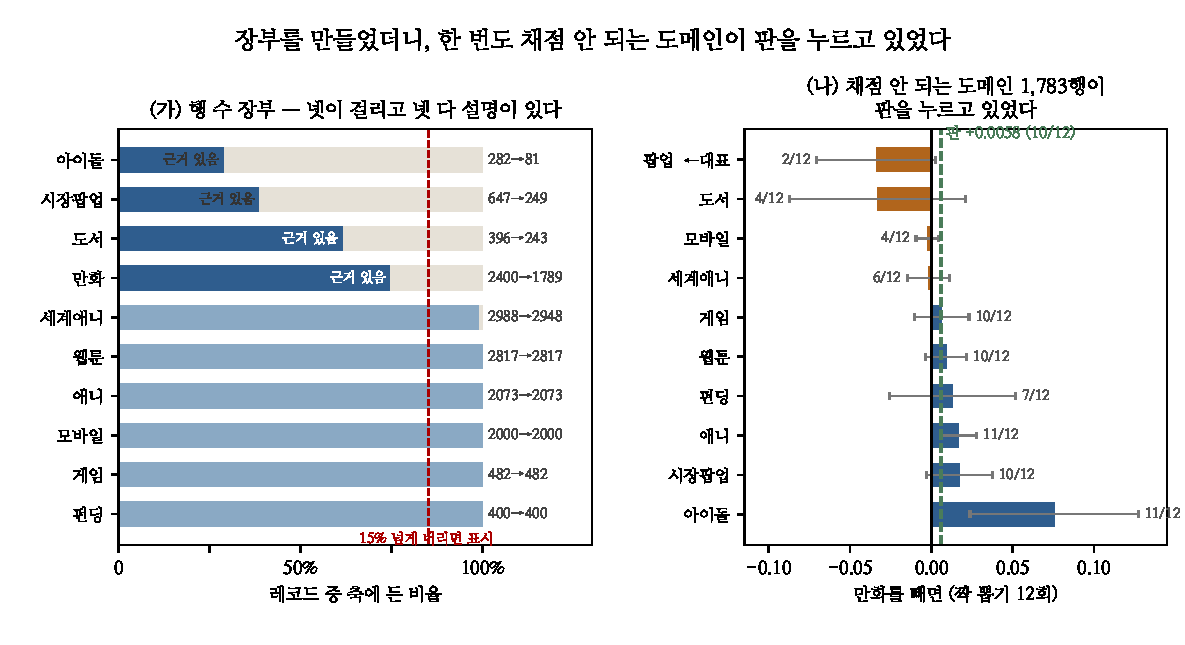
\includegraphics[width=\linewidth]{figs/ledger.pdf}\end{center}

장부는 도메인마다 두 수만 견준다. \textbf{판정하지 않는다} --- 버리는 데는
옳은 이유가 많다. 표시하고, 근거를 찾는 것은 사람 몫이다.

\begin{center}
\begin{tabular}{lrrrl}
\hline
도메인 & 레코드 & 축 & 버림 & 근거 \\
\hline
아이돌   &   282 &    81 & 71\% & \texttt{chodong} 결측 107 (idolset 은 173행을 직접 읽는다) \\
시장팝업 &   647 &   249 & 62\% & 단일 행사 아님 · 방문객 없음 (노트 354) \\
도서     &   396 &   243 & 39\% & 전자책 153 (노트 35 · 253) \\
만화     & 2,400 & 1,789 & 26\% & 비일본 611 (\texttt{KEEP\_COUNTRY}, 노트 79) \\
세계애니 & 2,988 & 2,948 &  1\% & --- \\
웹툰 · 애니 · 모바일 · 게임 · 펀딩 & & & 0\% & --- \\
\hline
\end{tabular}
\end{center}

\textbf{지금 돌리면 새로 나오는 것이 없다.} 노트 354가 마지막 구멍을
메웠기 때문이다. 값은 소급 검증에 있다 --- 노트 354 \emph{전에} 돌렸으면
시장팝업이 68\%로 제일 크게 걸렸을 것이고, 일곱 번을 운으로 찾는 대신
한 번에 봤을 것이다.

\textbf{정정 하나.} 처음에 만화를 ``어디에도 안 적혀 있다''로 적었는데
틀렸다. 노트에 없었을 뿐 \texttt{ingest/manga\_axes.py:118} 에 근거까지 다
있다 --- KR 556건은 자기 순위 상관이 $+0.083$ 으로 일본 작품($+0.477$)의
6분의 1이고, 라벨이 \emph{세계 독자}의 서재 등록 수라 한국 작품은 영어
번역 유무에 지배된다. \textbf{장부는 제 일을 했다} --- 표시했고, 읽어 보니
설명이 있었다.

\section{읽다가 나온 물음}

표를 보다 걸린 것은 버림이 아니라 다른 수였다. \textbf{만화는 학습
1,783행인데 유보가 6행이라 \texttt{evaluate} 의 문턱 20을 못 넘어 한 번도
채점되지 않는다.} 판 가중에도 안 들어간다. 그런데 학습에는 들어간다 ---
전체 학습 10,483행의 \textbf{17\%}다.

\textbf{채점 안 되는 도메인이 공유 적합에 무엇을 하는지 아무도 안 물었다.}
노트 252가 ``풀링은 타협이 아니라 이득''을 보였지만 그것은 \emph{채점되는}
도메인들 얘기였다. 빼 봤다 --- 열두 번 짝 뽑기.

\begin{center}
\begin{tabular}{lrrr}
\hline
만화를 빼면 & 차 & SD & 부호 \\
\hline
\textbf{판}   & $\mathbf{+0.0058}$ & 0.0058 & \textbf{10/12} \\
\hline
아이돌   & $+0.0754$ & 0.0517 & 11/12 \\
시장팝업 & $+0.0173$ & 0.0202 & 10/12 \\
애니     & $+0.0168$ & 0.0111 & 11/12 \\
펀딩     & $+0.0128$ & 0.0387 & 7/12 \\
웹툰     & $+0.0092$ & 0.0126 & 10/12 \\
게임     & $+0.0064$ & 0.0167 & 10/12 \\
세계애니 & $-0.0018$ & 0.0130 & 6/12 \\
모바일   & $-0.0027$ & 0.0068 & 4/12 \\
도서     & $-0.0331$ & 0.0542 & 4/12 \\
\textbf{팝업}(대표) & $\mathbf{-0.0340}$ & 0.0367 & 2/12 \\
\hline
\end{tabular}
\end{center}

$+0.0058$ 은 노트 349 · 350 · 351을 다 합친 것($+0.0079$)에 가깝다. 여덟
도메인 중 여섯이 오르고 아이돌은 $+0.0754$ 다.

\section{그런데 안 뺀다}

노트 275의 규칙은 이렇다. \textbf{①} 판이 미결정 폭($0.010$) 안이고
\textbf{②} 어느 도메인도 $|t| > 2.77$ 로 안 나빠지면, \textbf{배포 쪽
이득이 정한다.}

① 판 $+0.0058 < 0.010$ --- 미결정이다. ② 제일 나쁜 팝업이
$-0.0340/0.0367$ 로 $|t| = 0.93$ --- 문턱 안이다. \textbf{그래서 규칙은
``판이 정하지 못한다, 배포가 정하라''로 넘긴다.} 배포 수치는 팝업이고
팝업은 $-0.0340$(\textbf{2/12})이다. \textbf{안 뺀다.}

\textbf{노트 351과 방향이 정확히 반대이고 규칙은 같다.} 그때는 판이
$+0.0002$ 로 미결정이었고 팝업이 $+0.0168$(11/12)이라 넣었다. 지금은 판이
$+0.0058$ 로 미결정이고 팝업이 내려가서 안 뺀다. \textbf{규칙이 두 번 다
정했고 두 번 다 판이 아니라 배포가 정했다} --- 판이 미결정 폭 안에서
움직이는 한 판은 결재권이 없다.

\textbf{그리고 노트 352가 여기에도 걸린다.} 팝업 $-0.0340$ 의 SD 가
$0.0367$ 이다 --- \emph{못 가린다.} 판 $+0.0058$ 도 SD $0.0058$ 이다.
\textbf{이 결정은 못 가리는 둘 사이에서 규칙으로 갈랐다.} 규칙이 없었으면
어느 쪽이든 고를 수 있었고, 그게 규칙을 미리 적어 두는 이유다.

\section{만화는 나쁜 가운데 자리에 있다}

만화는 학습에 들어가고 채점에는 안 든다. 그 자리가 $+0.0058$ 짜리다.
나가는 문이 둘인데 둘 다 안 열려 있다.

\textbf{하나 --- 뺀다.} 판이 오르지만 대표가 내려가 규칙이 막았다.

\textbf{둘 --- 채점되게 만든다.} 문턱 20을 넘기려면 유보 20행이 필요한데
지금 6행이다. 버린 611건 중 2025년이 10건이라 다 넣어도 16행이고,
그나마 그 611건은 노트 79가 근거를 대고 뺀 것이다. \textbf{2026년 만화
레코드가 아예 없다} --- 긁어야 한다.

둘째가 옳은 문이다. 만화는 유일하게 ``자료는 많은데 최근이 없어서'' 못
재는 도메인이고, 2026년 것을 스무 건만 더 모으면 열한 번째 채점 도메인이
된다. \textbf{그것은 판을 $+0.0058$ 올리는 일보다 크다} --- 노트 352가
센 것처럼 지금 마흔다섯 쌍 중 스물아홉이 순서가 안 갈리는데, 도메인이
하나 더 서면 그 분모부터 바뀐다.

\section{규약에 더하는 줄}

\begin{itemize}
\item \textbf{목록 대조는 이름이 아니라 행으로 한다.} 도메인 이름이 양쪽에
있어도 행이 갈릴 수 있다 --- 노트 354가 그랬다.
\item \textbf{장부는 표시만 하고 판정하지 않는다.} 넷이 걸렸고 넷 다
근거가 있었다. 근거가 코드 주석에 있고 노트에 없어도 근거다.
\item \textbf{학습에만 들어가는 도메인은 따로 센다.} 만화 1,783행이
전체 학습의 17\%이고 판 $+0.0058$ 짜리인데, 그 도메인은 점수표에 한 줄도
안 나온다.
\end{itemize}

\section{남은 것}

\begin{center}
\begin{tabular}{ll}
\hline
갈래 & 지금 아는 것 \\
\hline
\textbf{만화 2026 스무 건} & 열한 번째 채점 도메인이 된다. \textbf{다음 순번} \\
만화가 왜 누르나 & 라벨 종류(선호형)로는 안 갈린다 --- 뺐을 때 \\
                & 선호형 웹툰 $+0.0092$ · 세계애니 $-0.0018$ 로 엇갈린다 \\
MKT2 나머지 195건 & 라벨 · 기간 없음. 원천 크롤에도 없다(107/338만 방문객) \\
추가 2026 아홉 행 & 노트 353. 아이돌 라벨 수준이 한터와 반대 \\
\hline
\end{tabular}
\end{center}

둘째 줄은 열어 둔다. ``왜 누르나''를 못 밝혔고, 라벨 종류 · 도메인 수 ·
행 수 중 무엇인지 가르려면 만화를 절반 · 4분의 1로 줄여 가며 재야 한다.
그건 판을 올리는 일이 아니라 아는 일이라 순번이 뒤다.

\end{document}
